\part{Pathfinding}
\frame{\partpage}

\begin{frame}{The problem}
    \begin{itemize}
        \item We have a \textbf{graph} \pause
            \begin{itemize}
                \item \textbf{Nodes} (points) \pause
                \item \textbf{Edges} (lines between points, each with a \textbf{length}) \pause
            \end{itemize}
        \item E.g.\ a road map \pause
            \begin{itemize}
                \item Nodes = addresses \pause
                \item Edges = roads \pause
            \end{itemize}
        \item E.g.\ a tile-based 2D game \pause
            \begin{itemize}
                \item Nodes = grid squares \pause
                \item Edges = connections between adjacent squares \pause
            \end{itemize}
        \item Given two nodes $A$ and $B$, find the \textbf{shortest path} from $A$ to $B$ \pause
            \begin{itemize}
                \item ``Shortest'' in terms of edge lengths --- could be distance, time, fuel cost, ...
            \end{itemize}
    \end{itemize}
\end{frame}

\begin{frame}{Applications of pathfinding}
    \begin{center}
        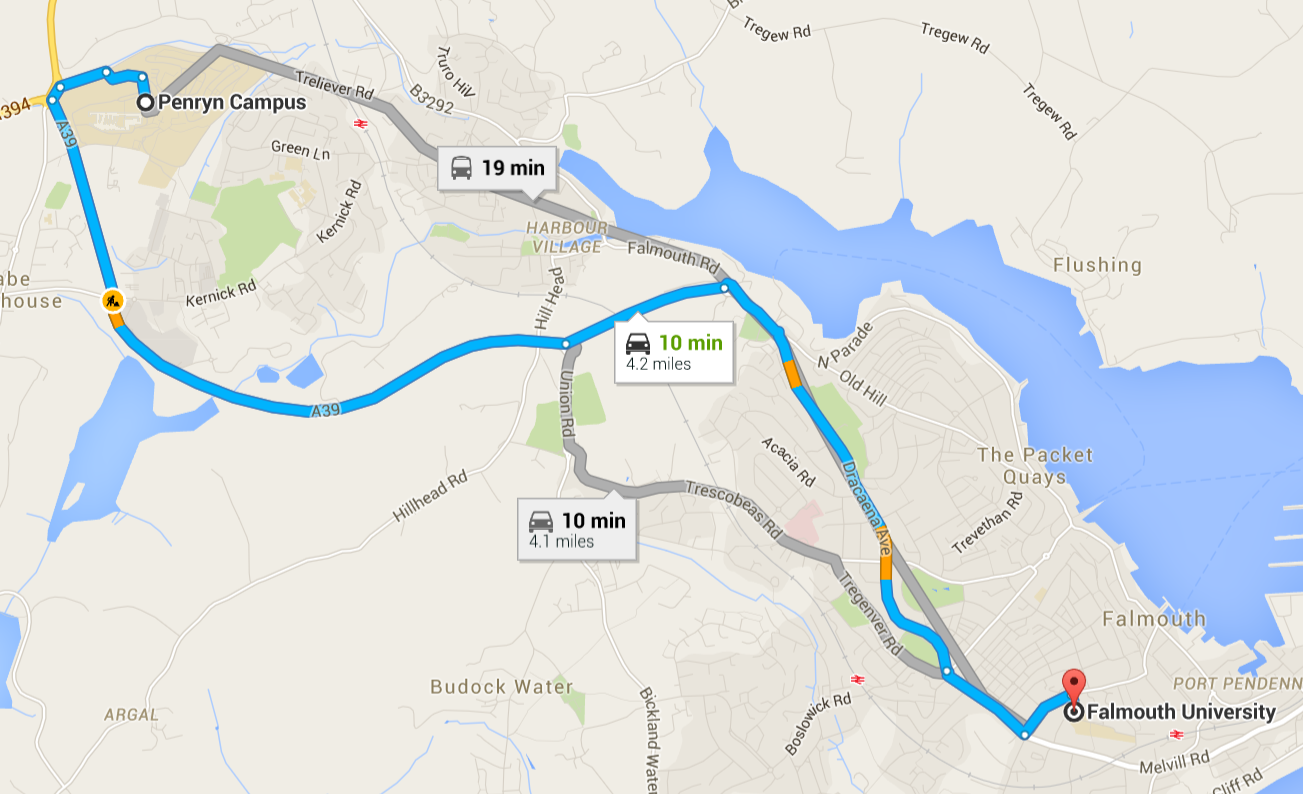
\includegraphics[width=\textwidth]{pathfinding_1}
    \end{center}
\end{frame}

\begin{frame}{Applications of pathfinding}
    \begin{center}
        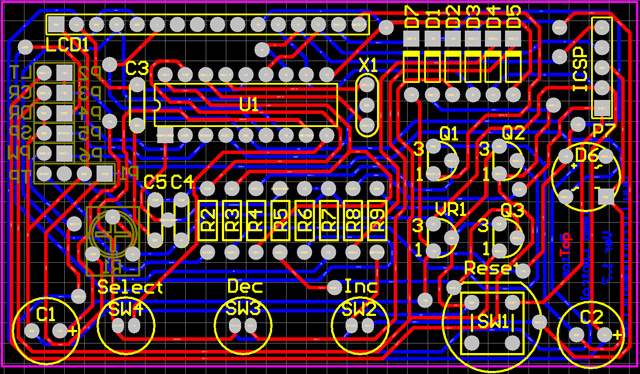
\includegraphics[width=\textwidth]{pcb}
    \end{center}
\end{frame}

\begin{frame}{Applications of pathfinding}
    Many applications in game AI \pause
    \begin{itemize}
        \item Non-player character AI \pause
        \item Mouse-based movement (e.g.\ strategy games) \pause
        \item Maze navigation \pause
        \item Puzzle solving
    \end{itemize}
\end{frame}

\begin{frame}{Pathfinding example}
    \begin{itemize}
        \pause\item \url{https://github.com/falmouth-games-academy/comp250-workshop-9}
        \pause\item Open it in PyCharm
    \end{itemize}
\end{frame}

\begin{frame}{Graph traversal}
	\begin{itemize}
		\pause\item \textbf{Depth-first} or \textbf{breadth-first}
		\pause\item Recall: can be implemented with a \textbf{stack} or a \textbf{queue} respectively
		\pause\item For graphs (as opposed to trees), need to remember which nodes have been \textbf{visited}
			to avoid getting stuck in a loop
		\pause\item Inefficient --- generally has to explore the \textbf{entire map}
		\pause\item Finds a path, but probably not the \textbf{shortest}
		\pause\item Third type of traversal: \textbf{best-first}
			\begin{itemize}
				\pause\item ``Best'' according to some heuristic evaluation
				\pause\item Often implemented with a \textbf{priority queue}
			\end{itemize}
	\end{itemize}
\end{frame}

\begin{frame}{Greedy search}
	\begin{itemize}
		\pause\item Always try to move \textbf{closer} to the goal
		\pause\item Visit the node whose \textbf{distance to the goal} is \textbf{minimal}
		\pause\item Doesn't handle \textbf{dead ends} well
		\pause\item Not guaranteed to find the \textbf{shortest} path
	\end{itemize}
\end{frame}

\begin{frame}{Dijkstra's algorithm}
	\begin{itemize}
		\pause\item Let $g(x)$ be the distance of the path found from the start to $x$
		\pause\item Choose a node that minimises $g(x)$
		\pause\item Needs to handle cases where a shorter path to a node is discovered later in the search
		\pause\item \textbf{Is} guaranteed to find the shortest path
		\pause\item ... but is not the most efficient algorithm for doing so
	\end{itemize}
\end{frame}

\begin{frame}{A$^*$ search}
    \begin{itemize}
    	\pause\item Let $h(x)$ be an estimate of the distance from $x$ to the goal (as in greedy search)
    	\pause\item Let $g(x)$ be the distance of the path found from the start to $x$ (as in Dijkstra's algorithm)
    	\pause\item Choose a node that minimises $g(x) + h(x)$
    \end{itemize}
\end{frame}

\begin{frame}{Properties of A$^*$ search}
    \begin{itemize}
        \item A$^*$ is \textbf{guaranteed} to find the shortest path
            if the distance estimate $h(x)$ is \textbf{admissible} \pause
        \item Essentially, \textbf{admissible} means it must be an \textbf{underestimate} \pause
            \begin{itemize}
                \item E.g.\ straight line Euclidean distance is clearly an underestimate
                    for actual travel distance \pause
            \end{itemize}
        \item The more accurate $h(x)$ is, the more efficient the search \pause
            \begin{itemize}
                \item E.g.\ $h(x) = 0$ is admissible (and gives Dijkstra's algorithm), but not very helpful \pause
            \end{itemize}
        \item $h(x)$ is a \textbf{heuristic} \pause
            \begin{itemize}
                \item In AI, a heuristic is an estimate based on human intuition \pause
                \item Heuristics are often used to prioritise search,
                    i.e.\ explore the most promising options first
            \end{itemize}
    \end{itemize}
\end{frame}

\begin{frame}{Tweaking A$^*$}
	\begin{itemize}
		\pause\item Can change how $g(x)$ is calculated
			\begin{itemize}
				\pause\item Increased movement cost for rough terrain, water, lava...
				\pause\item Penalty for changing direction
			\end{itemize}
		\pause\item Different $h(x)$ can lead to different paths (if there are multiple ``shortest'' paths)
	\end{itemize}
\end{frame}

\begin{frame}{String pulling}
	\begin{itemize}
		\pause\item Paths restricted to edges can look unnatural
		\pause\item Intuition: visualise the path as a string, then pull both ends to make it taut
		\pause\item Simple algorithm:
			\begin{itemize}
				\pause\item Found path is $p[0], p[1], \dots, p[n]$
				\pause\item If the line from $p[i]$ to $p[i+2]$ is unobstructed, remove point $p[i+1]$
				\pause\item Repeat until there are no more points that can be removed
			\end{itemize}
	\end{itemize}
\end{frame}

